% !TeX spellcheck = italian
\documentclass[12pt,italian]{report}
\usepackage{tesi}

\usepackage[a4paper]{geometry}		% Formato del foglio
\usepackage[italian]{babel}			% Supporto per l'italiano
\usepackage[utf8]{inputenc}			% Supporto per UTF-8
%\usepackage[a-1b]{pdfx}				% File conforme allo standard PDF-A (obbligatorio per la consegna)

\usepackage{graphicx}				% Funzioni avanzate per le immagini
\usepackage{hologo}					% Bibtex logo with \hologo{BibTeX}
\usepackage{epsfig}				    % Permette immagini in EPS
\usepackage{xcolor}                 % Gestione avanzata dei colori
\usepackage{amssymb,amsmath,amsthm} % Simboli matematici
\usepackage{listings}				% Scrittura di codice
\usepackage{url}					% Visualizza e rendere interattii gli URL
\usepackage[pdfa]{hyperref}			% Rende interattivi i collegamenti interni
\usepackage{tikz}                   % Permette di disegnare inline
\usepackage{import}
\usepackage{float}
\usepackage{xstring}                % Permette di usare la funzione \IfInteger
\usepackage{array}                  % Permette di usare colonne "m" dentro table
\usepackage{multirow}               % Permette di creare tabelle con righe multiple
\usepackage{caption}                % Roba per le figure side-by-side
\usepackage{subcaption}             % Roba per le figure side-by-side
\graphicspath{{immagini/}}

\usetikzlibrary{positioning}
\usetikzlibrary{calc}
\usetikzlibrary{shapes}

\usepackage[autostyle = false]{csquotes}
\MakeOuterQuote{"}

\newcommand{\GeneraSchemaPacchetto}[2]{{
\begin{tikzpicture}
    [
        box/.style={draw,rectangle,minimum width=\recminwidth, 
        minimum height=\rectangleheight, 
        outer sep=0pt, node distance=0pt}
    ]

    \def\rectangleheight{1cm}
    \def\recminwidth{2cm}

    \foreach \name/\size in {#1} {
        \node[box, label={below:\small \texttt{\size{} byte}}] (0) {\texttt{\name}};
    }    

    \foreach \name/\size [count=\i] in {#2}
    {
        \pgfmathtruncatemacro\prevposition{\i - 1}
        \node[box, right = 0pt of \prevposition,
            label={below:\small \texttt{\IfInteger{\size}{\size\ byte}{\size}}}
        ] (\i) {\texttt{\name}};
    }
\end{tikzpicture}
}}

\def\myCDL{Corso di Laurea in\\ Sicurezza dei Sistemi e delle Reti Informatiche}

% TITOLO TESI:
\def\myTitle{VirTEE: implementazione di un protocollo per la condivisione TEE in Cloud}

% AUTORE:
\def\myName{Massimo Perego}
\def\myMat{Matr. Nr. 965229}

% RELATORE E CORRELATORE: 
\def\myRefereeA{Prof. Andrea Lanzi}

% ANNO ACCADEMICO
\def\myYY{2022-2023}

% Il seguente comando introduce un elenco delle figure dopo l'indice (facoltativo)
%\figurespagetrue

% Il seguente comando introduce un elenco delle tabelle dopo l'indice (facoltativo)
%\tablespagetrue

\begin{document}

	\frontespizio
	\afterpreface

	\chapter*{Sommario}
	\addcontentsline{toc}{chapter}{Sommario}  
	\label{cap:sommario}
	
	\chapter{Introduzione}
	\label{sec:introduzione}
	
	\chapter{Trusted Execution Environment}
	\label{cap:TEE}
	Un \textit{Trusted Execution Environment} (TEE) è un'area isolata e sicura all'interno di un dispositivo, concepita con l'intento di operare in modo affidabile ed indipendente dal resto del sistema operativo. Questo permette di ospitare applicazioni e processi sensibili, eseguendo unicamente codice autenticato.
	
	I TEE stanno progressivamente guadagnando maggiore rilevanza in virtù del loro impiego per l'arricchimento di piattaforme preesistenti, offrendo soluzioni atte a incrementare la sicurezza e prevenire accessi o manipolazioni non autorizzate. Grazie a tali caratteristiche, i TEE trovano utilizzo in diverse applicazioni e ambiti operativi.
	
	\bigbreak
	
	I TEE sono presenti sulla maggioranza dei cellulari tramite nomi quali \textit{TrustZone} di ARM, \textit{Samsung Knox}, \textit{Qualcomm QTEE}, \textit{Google Titan M} e \textit{Apple Secure Enclave}, con più finalità, tra le quali: autenticazione sicura, gestione di chiavi crittografiche e gestione dei diritti digitali.
	
	L'impiego dei TEE però sta assumendo un ruolo crescentemente significativo non solo nell'ambito dei dispositivi mobili, ma anche nei settori Desktop, Server e IoT. Sono sempre più numerosi i prodotti sul mercato che consentono esecuzione di codice sicuro anche in tali ambienti. Tale tendenza riflette la crescente preoccupazione per la sicurezza informatica e la protezione dei dati sensibili in un'ampia gamma di applicazioni e scenari operativi.
	
	In questo capitolo verranno esplorate le principali caratteristiche dei TEE e come tali implementazioni possano contribuire a migliorare l'affidabilità di vari tipi di sistemi.
	
	\newpage
	
	\section{TEE GlobalPlatform}
	\label{sec:GlobalPlatform}
	%Deve contenere: cos'è globalplatform, architettura, cosa ne consegue (che sicurezza e cosa forniscono)
	Il concetto di "Trusted Execution Environment" denota una combinazione di tecniche software e hardware progettate per creare un ambiente sicuro e protetto. Nonostante ciò, il termine risulta piuttosto generico, in quanto fa riferimento a una vasta gamma di prodotti con caratteristiche implementative e livelli di sicurezza diversi.
	
	L'assenza di standardizzazione potrebbe essere causa di confusione tra i consumatori e diventare un ostacolo per la portabilità ed interoperabilità di Trusted Applications (TA) su diverse implementazioni di TEE. Ciò implica la necessità di gestire una gamma di differenze nell'implementazione e garanzie di sicurezza offerte, complicando l'utilizzo di tali ambienti in modo uniforme e trasversale.
	
	A risoluzione di questi problemi il consorzio GlobalPlatform pubblica dei documenti contenenti specifiche che coprono vari aspetti chiave della realizzazione di TEE, favorendo l'interoperabilità tra dispositivi e sistemi.
	
	All'interno delle specifiche di GlobalPlatform, si possono trovare direttive dettagliate relative a diverse tematiche riguardanti i Trusted Execution Environments, tra le quali: il modello architetturale dei TEE, delineando le sue componenti fondamentali, un insieme standard di interfacce API e metodi per la gestione sicura delle credenziali.
	
	\bigbreak
	
	Un altro aspetto trattato è l'istituzione di parametri e criteri per la valutazione della sicurezza dei TEE. Attraverso queste direttive, si mira a garantire che tali ambienti protetti soddisfino precisi standard di robustezza e affidabilità.
	
	Un numero sempre crescente di organizzazioni sta adottando questi standard e adeguando le proprie soluzioni alle specifiche GlobalPlatform. La tendenza generale è di una sempre più ampia adozione di TEE in conformità con queste direttive, pertanto questo elaborato farà riferimento a TEE conformi GlobalPlatform.
	
	\bigbreak 
	
	In generale, l'implementazione di un TEE conforme alle direttive di GlobalPlatform consente di garantire un elevato livello di sicurezza, interoperabilità e affidabilità del TEE su una vasta gamma di dispositivi e piattaforme, creando un ambiente di esecuzione sicuro per applicazioni sensibili e riservate.
	
	\newpage
	
	\subsection{Architettura TEE}
	\label{subsec:architettura}
 	Le direttive di GlobalPlatform non fanno riferimento ad implementazioni specifiche per quanto riguarda l'architettura, ma piuttosto delineano una struttura generale degli elementi logici costituenti il TEE e le loro interazioni. Vengono solamente stabiliti i requisiti di sicurezza che l'hardware deve poter garantire al TEE.
 	
 	\bigbreak
 	
 	In generale, il sistema è suddiviso in due ambienti distinti, noti come \textit{Trusted Execution Environment} (TEE) e \textit{Regular Execution Environment} (REE). Quest'ultimo costituisce l'insieme dei componenti di un dispositivo e il sistema operativo convenzionale. Generalmente si ha un solo TEE, ma nulla vieta di implementarne molteplici, sebbene si tratti di una pratica poco comune. Da qui in poi si farà riferimento ad un ambiente con un solo TEE e REE per semplicità.
 	
 	Ogni risorsa può essere controllata dal REE o da un TEE ed il possesso può essere trasferito tra gli ambienti. Una risorsa controllata da uno specifico TEE viene isolata dagli altri ambienti di esecuzione, se non altrimenti specificato esplicitamente dal TEE. In generale, il TEE può avere capacità di accedere alle risorse del REE, mentre il contrario non è possibile, a meno che non siano concessi permessi specifici. 
 	
 	L'unico modo che il REE ha per accedere alle risorse in ambiente protetto è tramite entry point delle API o servizi esposti dal TEE, ma non viene specificato un metodo preciso per imporre il controllo degli accessi.
 	
 	\begin{figure}
 		\centering
 		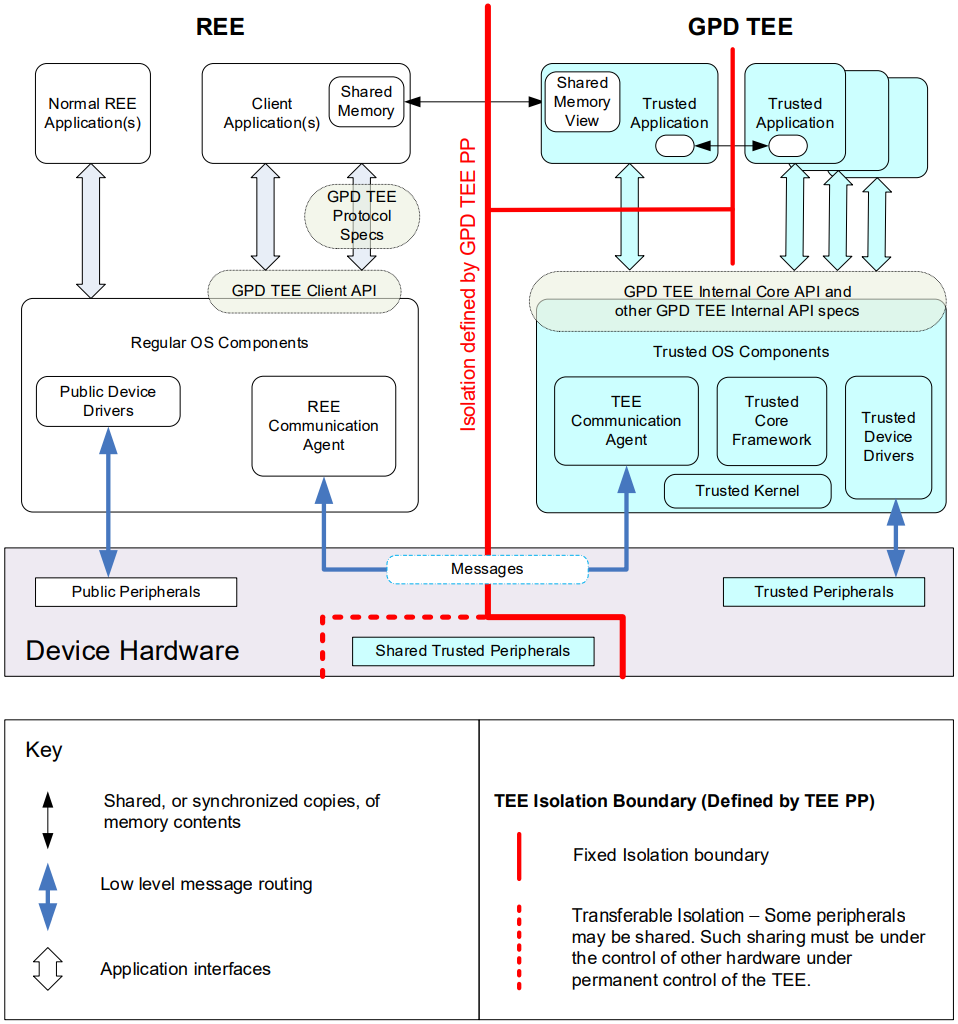
\includegraphics[width=1\textwidth]{immagini/TEE_SW_Architecture}
 		\caption{
 			Architettura di un TEE conforme GlobalPlatform. 
 			Da \textit{TEE System Architecture v1.3 (pag. 28)}
 			\cite{gp2020systemarchitecture}
 		}
 		\label{fig:tee-architecture}
 	\end{figure}
 	
 	\bigbreak
 	
 	In \figurename~\ref{fig:tee-architecture} si può vedere un possibile esempio di architettura software di un sistema conforme GlobalPlatform. Si può vedere la separazione di REE e TEE, in quanto ambienti completamente separati, dotati ciascuno di sistema operativo, scheduling e risorse proprie.
 	
 	Le applicazioni all'interno del REE vengono classificate come \textit{Client Applications} (CA), mentre le applicazioni all'interno del TEE sono denominate \textit{Trusted Applications} (TA).
 	
 	All'interno del TEE è presente un \textit{Trusted Kernel} che fornisce scheduling ed altre funzioni di gestione del sistema operativo, sia per le TA che per il Trusted Core Framework.
 	
 	\bigbreak
 	
 	Una CA per richiedere un servizio da una Trusted Application utilizza la \textit{Client API}. Tale API consente di stabilire una sessione con la TA e inviare un messaggio contenente la funzione da invocare e i relativi parametri.
 	
 	All'interno di entrambi gli ambienti sono presenti dei \textit{Communication Agent}. Questi agenti si occupano di fornire il supporto per lo scambio di messaggi tra la Client Application e la Trusted Application e, se necessario, anche tra diverse TA.
 	
 	
 	\paragraph{Trusted Core Framework:} le Trusted Application possono fare uso della \textit{Trusted Core Framework API}, la quale definisce API ed infrastrutture simili a quelle presente in un sistema operativo. Ciò permette di avere un'interfaccia comune per le TA, indipendentemente dal TEE sulla quale vengono eseguite. Queste specifiche sono contenute all'interno del \textit{TEE Internal Core API Specification}\cite{gp2020internalapi}.
 	
 	\paragraph{Periferiche:} vengono suddivise in tre categorie: 
 	\begin{itemize}
 		\item \textit{Public Peripherals}: possono essere utilizzate sia dal TEE che dalle applicazioni REE. L'accesso dalle TA avviene attraverso API fornite dal TEE. L'utilizzo da parte di applicazioni esterne al TEE segue le modalità di accesso standard del sistema operativo.
 		\item \textit{Trusted Peripherals}: l'accesso a questo periferiche è consentito esclusivamente a TA autorizzate, tramite interfacce API definite dal TEE.
 		\item \textit{Shared Trusted Peripherals}: di norma l'accesso a queste periferiche è consentito solo al TEE, ma questo può concedere temporaneamente l'accesso anche al REE. Il processo di condivisione deve essere comunque gestito da hardware sotto il controllo del TEE.
 	\end{itemize}
 	
 	
 	\subsection{Garanzie di Sicurezza}
 	\label{subsec:garanzie}
 	Come già detto in precedenza, il termine "Trusted Execution Environment" può fare riferimento ad una moltitudine di prodotti, quindi questi potrebbero variare in termini di garanzie di sicurezza che forniscono. Per questo motivo GlobalPlatform ha definito all'interno del \textit{Protection Profile} \cite{gp2020protectionprofile} i requisiti minimi di sicurezza che un TEE deve avere per poter essere certificato. Nonostante le proprietà indicate rappresentino una linea base minima, non è detto che un TEE non possa implementarne altre.
 	
 	\bigbreak
 	
 	In generale si può affermare che un TEE dovrebbe garantire le proprietà di integrità e confidenzialità del codice e di ciò che esso crea, e garantire esecuzione isolata rispetto al REE.
 	
 	Come già visto per altri documenti, GlobalPlatform non stabilisce implementazioni precise ma fornisce solo delle direttive. Nonostante ciò, all'atto pratico si hanno alcune caratteristiche comuni alla maggior parte dei TEE, come l'utilizzo di firme digitali per l'autenticazione del codice e l'utilizzo di supporto hardware per realizzare l'isolamento.
 	
 	\paragraph{Isolamento:}
 	
 	\paragraph{Integrità e autenticità:}
 	
 	\section{Applicazioni dei TEE}
 	\label{sec:applicazioni}
	
	\section{Supporto Hardware per i TEE}
	\label{sec:supporto-hw}
	Da scrivere tutti i tipi di TEE (quelli scritti sopra, sgx, sev, trustzone, processori dedicati, TEE RISC-V) ed il relativo hardware
	
	\section{Vulnerabilità Comuni}
	\label{sec:vulnerabilità}
	
	
	
	\chapter{TEE in Ambiente Cloud}
	\label{cap:problema}
	Virttee design problems, problema nel portare roba in cloud e come risolverli. Problematiche e come sono state affrontate. Componenti senza implementazione, mettere schemi di funzionamento
	
	
	
	\chapter{Sicurezza dei Dati}
	\label{cap:implementazione}
	Nome WIP. Dettagli riguardo all'implementazione, soluzioni tecniche trovate
	%Iniziare con ciò che ha fatto marco? 
	%Section del capitolo prima?
	
	
	
	\chapter{Analisi Performance}
	\label{cap:dati}
	%Riportare performance generali del sistema, dati di Marco
	%Analisi performance con l'implementazione
	%Commentare i risultati, perché alcuni sono 4% altri 150%
	
	\chapter{Conclusioni}
	\label{cap:conclusioni}
	%Lavori futuri e conclusioni
	
	\bibliographystyle{unsrt}
	\bibliography{bibliografia}
	\addcontentsline{toc}{chapter}{Bibliografia}

\end{document}
